\chapter{神经网络的泛化}
\label{chap:neural-network-generalization}

识别器在训练图像上都给出正确类别，遇到新的背景或主体时，两个网络却可能作出不同预测。它们可能分别依赖物体形状和背景线索，训练准确率没有显示这份差异。增加训练时间、改变初始化或增强方式，又可能改变学得的线索。泛化分析因此要把样本覆盖、网络采用的规律与未来使用条件联系起来。

训练损失评价已经观察到的样本，未来风险评价实际使用中的新输入。本章沿数据、候选函数与选解过程说明怎样改善后者：增强给出更多训练条件，结构与显式损失规定候选和评价偏好，更新与轨迹选择决定从中学得哪个解，集成再组合多个预测。每种方法的机制、条件和成本都接到它改变的对象上。

记参数为$\bm\theta$，训练集为$S=\{(\bm x_i,y_i)\}_{i=1}^n$，未来样本分布为$P$。经验风险与期望风险分别为
\begin{equation}
  \hat R_S(\bm\theta)=\frac1n\sum_{i=1}^n
    \ell(f_{\bm\theta}(\bm x_i),y_i),\qquad
  R_P(\bm\theta)=\mathbb E_{(\bm x,y)\sim P}
    [\ell(f_{\bm\theta}(\bm x),y)]\text{。}
  \label{eq:generalization-risks}
\end{equation}
后面的控制手段以未来预测为目标。$R_P-\hat R_S$描述经验评价与未来评价之间的差距；两处都表现很差的常量模型，也可能有很小差距。增强强度、正则化系数与停止时刻由独立验证数据选择，最终测试再评估已确定的方案。

\section{主要挑战}
\label{sec:generalization-challenges}

训练数据可能只覆盖少数背景和主体，结构又可能强制共享本应不同的规则；即使有多个同样拟合的解，更新也可能选择对新输入不适用的线索。下面按这些失败的来源说明控制手段。复杂度分析考察候选范围，稳定性分析连接样本变化与所得预测，二者为这里的机制提供不同条件（参考\BookSectionRef{sec:deep-theory-comparison}{第二卷“基础、理论和可信性”的理论比较节}）。

\subsection{数据不足与数据质量}
\label{sec:generalization-data-quality}

训练中某类物体总与同一种背景出现时，识别器可以用背景区分类别。这个规则符合已有样本，却可能在更换背景后失效。经验风险只评价已经出现的条件，因此增强与正则化要先对应缺失的类别、环境、主体或时间范围，再决定补充什么约束。相同总样本数可以具有不同覆盖。

标注错误还会把错误监督带进经验目标。近似随机错误与集中在某类样本的系统性错误，会约束不同输入上的预测。重复记录增加样本行数，但来自同一主体的相关窗口可能仍共享同一份证据。独立同分布分析以真实抽样单位为参照，例如独立主体而非其每个窗口（参考\BookChapterRef{chap:statistical-learning-framework}{第二卷“基础、理论和可信性”的“机器学习理论基础”章}）。

\term{同分布泛化}（in-distribution generalization）考察来自与训练采样相同分布的新样本；\term{分布变化}（distribution shift）则涉及未来输入、标签机制或二者关系发生改变。同分布风险的结论依赖原采样分布，分布改变后还要检查相应条件。增强模拟指定变化，覆盖范围由所选变换决定。主体、时间或场景相关数据按预期使用方式划分，使验证与测试体现真正的新条件。

\subsection{模型容量与归纳偏置}
\label{sec:generalization-capacity}

能拟合复杂关系的网络，也可能将固定背景或错误标签拟合进去。\term{模型容量}（model capacity）描述候选函数族能够实现多丰富的函数或判别行为，参数数目提供其中一个规模指标。层间共享、激活与允许的权重范数规定这个范围，输入分布和学习算法再影响哪些差异会被观察和采用。模型族与样本量需要共同进入风险分析（参考\BookSectionRef{sec:network-learning-problem}{第二卷“基础、理论和可信性”的“深度学习的可学习性”章“神经网络的学习问题”节}）。

\term{归纳偏置}（inductive bias）是模型与学习方法倾向于采用哪些规律的先验偏好。卷积倾向复用局部模式，循环共享倾向使用同一状态更新，注意力的可见性和位置表示规定哪些交互可以发生。偏好与任务吻合时，模型直接复用所需结构；任务在不同位置需要不同规律时，共享反而可能排除合适函数。

网络范数可以和输入尺度、损失及分类间隔一起进入泛化上界，给定条件下限制函数变化或复杂度（参考\BookSectionRef{sec:network-norm-bounds}{第二卷“基础、理论和可信性”的“深度学习的可学习性”章“基于参数大小的可学习性”节}）。约束过强可能妨碍拟合，过弱则可能保留无关自由度。代表性验证数据用来比较这种取舍的实际预测结果。

\subsection{解选择与训练敏感性}
\label{sec:generalization-solution-selection}

同一批样本可以被多个预测函数拟合，更新规则决定轨迹更倾向哪一个。初始化、抽样、次序和优化器参与这一选择，未见数据的预测也可能随之改变（参考\BookSectionRef{sec:implicit-bias}{第二卷“基础、理论和可信性”的“深度学习的可学习性”章“基于参数梯度更新的可学习性”节}）。这里把训练数据或训练随机性的小变化引起所得预测明显变化称为\term{训练敏感性}（training sensitivity）；扰动发生在学习过程，输入扰动敏感性则考察已固定的模型。

正则化偏好某些解，提前终止选择较早状态，参数平均综合轨迹，集成组合预测；它们都在已有训练拟合之外增加选择机制。算法稳定性进一步考察更换一个训练样本后输出损失怎样变化，在规定假设下把过程敏感性与风险连接起来（参考\BookSectionRef{sec:algorithmic-stability}{第二卷“基础、理论和可信性”的“一般学习的可学习性”章“算法稳定性与可学习性”节}）。实际随机种子实验提供当前设置的经验差异，形式化界还需要相应采样与算法条件。

表~\ref{tab:generalization-challenge-remedies}将数据缺口、结构失配和选解波动接到后面的控制手段。作用对象与适用条件一起列出，便于按当前失败选择机制。
\begin{table*}[htbp]
\centering\small
\begin{tabular}{@{}p{32mm}p{48mm}p{27mm}p{48mm}@{}}
\toprule
挑战 & 作用机制与方法 & 后续内容 & 适用边界\\
\midrule
场景覆盖不足、伪相关 & 用合法变换、样本混合补充经验约束 & 第\ref{sec:generalization-augmentation}节 & 变换须保持或同步改变目标；不创造独立观测\\
函数范围与目标失配 & 共享、结构选择与显式惩罚改变候选或偏好 & 第\ref{sec:generalization-constraints}节 & 约束不能删除目标所需规律\\
噪声拟合与选解波动 & 扰动、提前停止、参数平均和模型集成 & 本章训练侧控制与集成各节 & 用独立验证确定强度；相关模型未必互补\\
主体相关与分布变化 & 按主体、时间或环境划分并检验变化 & 本节与各方法评估 & 同分布风险界不能直接保证域外风险\\
\bottomrule
\end{tabular}
\caption{从泛化挑战选择控制手段。各方法的作用对象与条件同时列出；一次失败也可能需要处理多个环节。}
\label{tab:generalization-challenge-remedies}
\end{table*}

\section{数据增强}
\label{sec:generalization-augmentation}

一个物体在不同位置、大小或光照下仍可能具有相同类别，分割位置则应随物体共同移动。数据增强将这些任务约定变为训练条件，要求共享模型在不同视图上满足相应监督。原样本提供内容，变换提供先验，增加的视图仍依赖原样本；这与第\ref{sec:generalization-capacity}节的归纳偏置相接。

\subsection{基于变换的数据增强}
\label{sec:generalization-transform-augmentation}

对任务允许的平移，分类标签可以保持，像素标签则同步移动。\term{数据增强}（data augmentation）按任务约定变换或组合已有样本，将这些关系加入经验目标。它增加指定条件下的预测约束；第\ref{sec:training-curvature}节的曲率则由改变后的完整目标决定。设随机变换为$T_{\xi}$，对应目标变换为$U_{\xi}$，增强后的目标为
\begin{equation}
  \hat R_{\mathrm{aug}}(\bm\theta)
  =\frac1n\sum_i\mathbb E_{\xi}
    [\ell(f_{\bm\theta}(T_{\xi}(\bm x_i)),U_{\xi}(y_i))]\text{。}
  \label{eq:generalization-augmentation-risk}
\end{equation}
分类中的保持标签变换令$U_{\xi}(y)=y$；分割中移动图像则需同步移动标签，表达输出随输入共同变换的等变关系。同一个原样本产生的视图共同依赖其内容，增加的是指定变换下的训练条件。

图像中的平移、裁剪、翻转和颜色调整，时间序列中的时间移位、局部扰动或伸缩，都需要按语义检查。例如，左右翻转不一定保持方向标签，裁剪可能移除识别对象，颜色变化可能破坏诊断所需信号，时间反转可能改变动作类别。这些例子中的目标随任务语义确定，同一变换在不同任务中可有不同标签关系。

增强强度规定训练要覆盖多远的变化。弱变换可能只重复已有条件，强变换则可能裁掉对象或改变答案。训练可以随机生成视图，验证按确定的使用条件评估；多次增强后平均预测会增加推理，应把它计入执行成本。尺度、字典或变换参数从训练集估计，后续评价沿用已确定的规则。

\subsection{基于样本混合的数据增强}
\label{sec:generalization-sample-mixing}

只在已有样本附近训练时，样本之间的预测关系仍缺少约束。混合增强把插值或区域组合交给同一个模型，为组合输入规定监督。\term{Mixup}用输入和监督目标的凸组合训练模型。对输入$\bm x_i,\bm x_j$及独热类别向量$\bm y_i,\bm y_j$，令$\lambda\sim\operatorname{Beta}(a,a)$，$a>0$，构造
\begin{equation}
  \tilde{\bm x}=\lambda\bm x_i+(1-\lambda)\bm x_j,\qquad
  \tilde{\bm y}=\lambda\bm y_i+(1-\lambda)\bm y_j\text{。}
  \label{eq:generalization-mixup}
\end{equation}
交叉熵对目标向量线性，因此混合目标的损失等于$\lambda\ell(f(\tilde{\bm x}),\bm y_i)+(1-\lambda)\ell(f(\tilde{\bm x}),\bm y_j)$。混合比例进入监督，因而对样本之间的预测施加插值偏好；输入是人为组合的训练条件\scite{zhang2018mixup}

\term{CutMix}从一个样本保留部分区域，用另一个样本的对应区域替换。设二值空间掩码$\bm M$在保留区域为1，则$\tilde{\bm x}=\bm M\odot\bm x_i+(\bm1-\bm M)\odot\bm x_j$，目标仍用凸组合，但$\lambda$取实际保留面积占比。面积按实际替换区域计算，裁到图像边界外的部分已不参与输入\scite{yun2019cutmix}

图~\ref{fig:generalization-mixing}用$2\times2$构造输入比较混合方式。Mixup使每个位置叠加，CutMix保留各区域的原始局部值。分类标签用面积作为组合权重，这是监督构造，实际类别证据还取决于可见对象。逐像素分割则用同一掩码组合标签，使每个位置对应其输入来源。
\begin{figure*}[htbp]
  \centering
  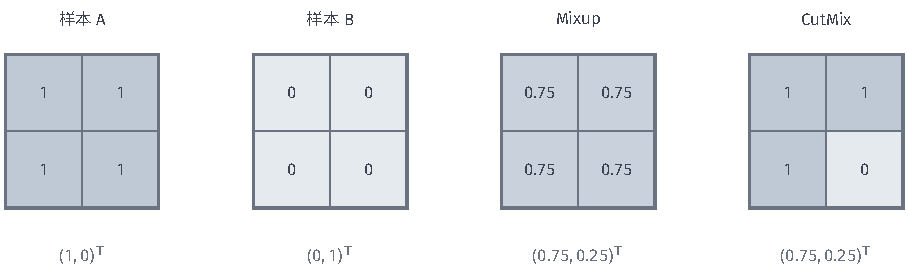
\includegraphics[width=153.793mm]{figures/05-neural-network-models/00-shared/tikz/generalization-mixing/figure.pdf}
  \caption{构造的两类$2\times2$输入及其混合。样本A各位置为1，目标为$(1,0)^{\top}$；样本B各位置为0，目标为$(0,1)^{\top}$。Mixup取$\lambda=0.75$，各位置变为0.75；CutMix替换右下位置，保留面积也为0.75。二者目标均为$(0.75,0.25)^{\top}$，但空间组织不同。教学数值用于比较混合机制，类别也是构造的。}
  \label{fig:generalization-mixing}
\end{figure*}

混合强度、配对与目标共同规定这份函数约束。插值缺少任务意义时，线性标签会引入错误监督；类别线索集中在小区域时，面积也可能误表其贡献。保留真实任务语义的验证样本用来检验这些构造是否改善原任务。

\section{模型侧的泛化控制}
\label{sec:generalization-constraints}

同一结构的未绑定版本允许各位置分别选择参数，共享与绑定将其中某些自由度合并；范数惩罚则保留参数范围，在损失中增加尺度或稀疏偏好。前者规定可选计算，后者评价候选，两条路线分别接到第\ref{sec:generalization-capacity}节的归纳偏置与范数复杂度分析（参考\BookSectionRef{sec:network-norm-bounds}{第二卷“基础、理论和可信性”的“深度学习的可学习性”章“基于参数大小的可学习性”节}）。

这里按主要作用位置区分模型侧与训练侧：固定结构及显式损失项放在本节，更新收缩、随机训练扰动和轨迹选择放在第\ref{sec:generalization-training-process}节。方法在数学上可以联系，例如普通SGD中的L2梯度等价于特定收缩；具体实现据改变目标还是改变更新确定其作用位置。

\subsection{参数共享与参数绑定}
\label{sec:generalization-parameter-sharing}

相同局部关系出现在多个位置时，可以让这些位置共同估计一份规则。第\ref{sec:generalization-capacity}节的结构偏好在这里体现为参数相等：自由度减少，各次使用的梯度汇到同一参数，也同时要求这些位置采用同一变换。\term{参数共享}（parameter sharing）让不同计算位置使用同一参数对象。卷积核跨位置复用，循环权重跨时间复用；每次使用都贡献梯度，更新时累积到同一对象。\term{参数绑定}（weight tying）则强调多个模块的参数被限制为相等或具有指定对应关系，硬绑定常通过共享实现。

例如，词表嵌入矩阵$\bm E\in\mathbb R^{v\times d}$的第$j$行表示词元$j$，输出隐藏状态为$\bm h\in\mathbb R^d$时，可以绑定输出矩阵，令分数$\bm z=\bm E\bm h+\bm b$。这里要求输出隐藏宽度与嵌入宽度相容，输入和输出词表也有一致对应；不相容时需投影或另外定义绑定范围。绑定让同一词元的输入表示与输出判别共享信息，也减少独立参数，但同时施加两种职责可由同一表示承担的假设。

若不希望强制相等，可加入$\lambda\lVert\bm\theta_A-\bm\theta_B\rVert_2^2/2$，鼓励两组参数接近。有限$\lambda$下它们仍是两个参数对象，这是一种软约束。共享规定相等的参数结构，软约束在仍可不同的参数之间增加代价。任务若需要不同位置采用不同规则，过强绑定可能妨碍拟合。

\subsection{参数范数惩罚}
\label{sec:generalization-norm-penalties}

多组参数都能拟合已有样本时，可以在训练损失之外给它们不同评价。范数惩罚增加参数尺度代价，再与输入和分类间隔一起分析风险（参考\BookSectionRef{sec:network-norm-bounds}{第二卷“基础、理论和可信性”的“深度学习的可学习性”章“基于参数大小的可学习性”节}）。\term{范数惩罚}（norm penalty）将学习目标改为
\begin{equation}
  \min_{\bm\theta}\ \hat R_S(\bm\theta)+\lambda\Omega(\bm\theta),
  \qquad\lambda\geq0\text{。}
  \label{eq:generalization-regularized-objective}
\end{equation}
常见选择为$\Omega=\lVert\bm\theta\rVert_1$或$\Omega=\lVert\bm\theta\rVert_2^2/2$。后者惩罚范数的平方，实践中常简称L2正则化。它惩罚参数幅度，L1在0附近的非光滑形状则可以促成精确的零参数。

\begin{example}[L1与L2的收缩不同]
  \label{ex:generalization-shrinkage}
  对标量教学目标$\tfrac12(w-a)^2$，加入$\lambda w^2/2$后，最优解为$w=a/(1+\lambda)$；加入$\lambda|w|$后，最优解为$w=\operatorname{sign}(a)\max(|a|-\lambda,0)$。例如$a=0.4,\lambda=0.5$时，前者为$0.4/1.5$，后者为0。两个解析最优解显示惩罚形状的作用；神经网络的实际稀疏结果还取决于其目标与非光滑求解方法。
\end{example}

如果要一起选择或去掉一组参数，可以采用$\Omega(\bm\theta)=\sum_g\lVert\bm\theta_g\rVert_2$，其中组$g$可能对应某个特征、神经元或通道，必要时再按组大小加权。组范数对整组是否为0产生偏好，与逐参数L1的稀疏形态不同。组的边界、是否重叠与大小权重共同定义实际惩罚。

L1与组范数的零点不可微，近端更新常能更直接处理其非光滑部分；L2则有梯度$\lambda\bm\theta$。参数尺度还受重参数化影响，例如ReLU网络中某层放大、下一层相应缩小可能保留函数但改变参数惩罚。相同函数因表示方式而有不同惩罚，分析和实现因而需要共同固定约束对象。系数及偏置、归一化参数是否参与，再决定额外代价作用于哪些自由度。

\section{训练侧的泛化控制}
\label{sec:generalization-training-process}

候选和显式损失确定后，还要选择何时停止、使用轨迹中的哪个状态、怎样更新以及施加什么扰动。这些选择改变同一数据上的学习过程，训练敏感性与选解偏好分别解释其中部分机制（参考\BookSectionRef{sec:algorithmic-stability}{第二卷“基础、理论和可信性”的“一般学习的可学习性”章“算法稳定性与可学习性”节}和\BookSectionRef{sec:implicit-bias}{第二卷“基础、理论和可信性”的“深度学习的可学习性”章“基于参数梯度更新的可学习性”节}）。验证风险用于比较学得候选的新数据表现。

下面先讨论停止、平均与优化器选择，再讨论权重衰减和随机扰动。权重衰减在更新中收缩参数，因此归入训练侧；Dropout及噪声按训练时的操作位置归类，也可以从随机计算的期望损失理解。期望损失联系目标，操作位置联系实现，两种描述可以用于同一方法。

\subsection{提前终止}
\label{sec:generalization-early-stopping}

训练损失还在下降时，验证损失可能已经开始升高。此时可以把沿同一数据训练的时长作为候选选择；相应光滑与抽样条件下，训练时间和步长总量也会进入稳定性界（参考\BookSectionRef{sec:sgd-stability}{第二卷“基础、理论和可信性”的“一般学习的可学习性”章“凸学习问题的随机梯度下降”小节}）。\term{提前终止}（early stopping）根据验证数据选择训练时刻，将训练轨迹上的参数位置当作候选模型。它需要规定评估指标、检查间隔、最小改善量和容忍窗口，并保存出现最佳验证表现时的参数。

例如，每训练一个轮次计算一次验证损失，若连续$p$次检查都没有超过阈值的改善，就停止并恢复已保存的最优参数。恢复参数与使用停止时刻的参数不同；继续训练还需相应恢复优化器和调度状态。随机验证增强、Dropout未关闭或BatchNorm模式错误，都可能让停止判断混入无关噪声。

图~\ref{fig:generalization-early-stopping}展示可能出现的曲线形状。真实曲线可能有多个起伏，短期变差后还可能改善。容忍窗口据噪声、调度与目标选择，决定要为后续改善等待多少计算。
\begin{figure}[htbp]
  \centering
  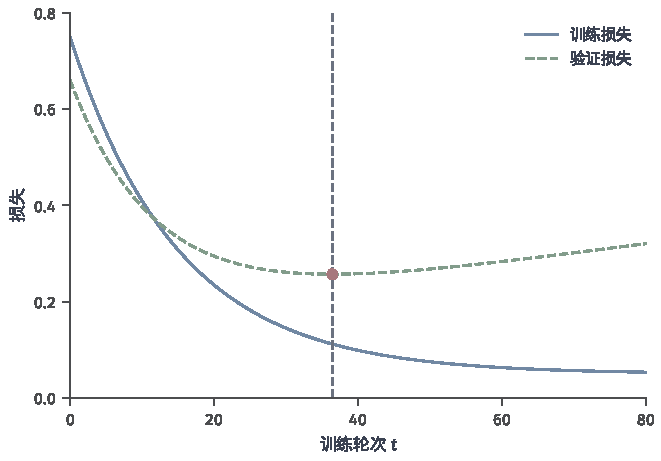
\includegraphics[width=105.412mm]{figures/05-neural-network-models/00-shared/matplotlib/generalization-early-stopping/figure.pdf}
  \caption{提前终止的示意曲线。训练损失取$0.05+0.7\exp(-t/15)$，验证损失取$0.16+0.5\exp(-t/12)+0.002t$，$t$为训练轮次。虚线标出该构造验证函数的极小点附近，说明继续拟合与验证表现可能分离；这些函数仅用于讲解，不是实验记录。}
  \label{fig:generalization-early-stopping}
\end{figure}

在特定光滑、Lipschitz等条件下，SGD的稳定性界与步长总量和训练时间联系，解释持续更新怎样累积对样本的依赖（参考\BookSectionRef{sec:sgd-stability}{第二卷“基础、理论和可信性”的“一般学习的可学习性”章“凸学习问题的随机梯度下降”小节}）。实际停止仍在拟合进展和验证风险之间选择\scite{hardt2016sgd}

反复尝试停止策略时，验证集也在参与模型选择，所得方案可能适应这组数据的偶然差异。方案确定后再用最终测试评价。时间序列与持续感知还要模拟实际状态保留，让每个评价时刻只用当时可见的信息。

\subsection{参数平均}
\label{sec:generalization-weight-averaging}

更新噪声可能使训练后段的参数在附近波动，某个瞬时位置因而未必代表整段轨迹。参数平均综合这些位置，最后仍形成一个可直接推理的模型；平均位置的损失和验证表现确定这份综合是否合适。第\ref{sec:training-inexact-gradients}节说明了这些波动的来源。\term{指数移动平均}（exponential moving average, EMA）维护$\bar{\bm\theta}^{(t)}=\rho\bar{\bm\theta}^{(t-1)}+(1-\rho)\bm\theta^{(t)}$，$\rho\in[0,1)$。取初值为训练初始参数或当前参数可以避免零初值的缩小效应，$\rho$越大，对近期变化的响应越慢。推理时使用平均参数形成一个模型。

\term{随机权重平均}（stochastic weight averaging, SWA）选取训练后段的多个参数状态作算术平均。对已收集的$k$个状态，加入新状态$\bm\theta$时更新$\bar{\bm\theta}_{k+1}=k\bar{\bm\theta}_k/(k+1)+\bm\theta/(k+1)$。原始方案利用较大或周期性学习率采样训练后段区域，平均后若使用BatchNorm，还需按平均模型重新估计运行统计量\scite{izmailov2018swa}

参数坐标的平均要先经过网络计算，预测平均则组合已有输出。非线性映射通常不满足$f_{(\bm\theta_A+\bm\theta_B)/2}=(f_{\bm\theta_A}+f_{\bm\theta_B})/2$。同一轨迹附近的参数具有较一致的坐标含义，平均可能仍处在低损失区；独立模型的隐藏单元置换或尺度差异则可能把平均送到其他函数。

\begin{example}[等价网络的参数平均可以失效]
  \label{ex:generalization-parameter-average}
  取无偏置的两单元ReLU网络$f(x)=\operatorname{ReLU}(x)+\operatorname{ReLU}(-x)=|x|$。网络A的输入权重为$(1,-1)$，输出权重为$(1,1)$；网络B只交换两个隐藏单元，输入权重为$(-1,1)$，输出权重仍为$(1,1)$。两个网络的函数完全相同，但逐坐标平均后的输入权重为$(0,0)$，输出恒为0。预测平均仍给出$|x|$。
\end{example}

EMA和SWA在训练参数之外维护一份平均参数，推理使用这一个函数。它们综合同一轨迹，独立训练模型的预测集成则使用另一组函数；平均位置的偏差与实际验证风险仍据该模型评价。

\subsection{优化算法的隐式偏差}
\label{sec:generalization-implicit-bias}

同一目标有多个低损失解时，更新方向使轨迹倾向其中某些解。\term{隐式偏差}（implicit bias）描述学习过程形成的这种选择偏好；小批量无偏则描述梯度估计的期望。即使损失没有附加惩罚，线性和矩阵学习中的更新也可以产生特定偏好（参考\BookSectionRef{sec:implicit-bias}{第二卷“基础、理论和可信性”的“深度学习的可学习性”章“基于参数梯度更新的可学习性”节}）。

可分线性二分类提供一个明确结果：对$y_i\in\{-1,1\}$、无显式惩罚的逻辑损失，在相应步长与可分条件下，梯度下降使$\lVert\bm w\rVert_2$不断增长，方向趋向欧氏最大间隔分隔方向。这份经验逻辑损失的下确界为0，有限范数下达不到它；更新仍选择特定方向（条件与推导参考\BookSectionRef{sec:implicit-bias}{第二卷“基础、理论和可信性”的“深度学习的可学习性”章“基于参数梯度更新的可学习性”节}）\scite{soudry2018implicit}

\begin{example}[改变更新几何会改变选出的解]
  \label{ex:generalization-update-geometry}
  用一个训练样本拟合$w_1+2w_2=1$，目标为$\tfrac12(w_1+2w_2-1)^2$。从零初始化出发，足够小的固定步长梯度下降始终沿$(1,2)^{\top}$移动，收敛到$(1/5,2/5)^{\top}$，这是欧氏最小范数解。若改为固定预条件$\bm P=\operatorname{diag}(4,1)$，更新始终沿$(4,2)^{\top}$移动，则收敛到$(1/2,1/4)^{\top}$。两个解的训练误差都为0，后者最小化的是$\bm w^{\top}\bm P^{-1}\bm w$。未来数据若需要不同坐标承担不同作用，二者的风险也可能不同，哪种偏好适用要由未来输入与目标关系决定。
\end{example}

深度网络的选解偏好还随参数化、初始化、学习率、批量与时长改变，优化器比较因而需要固定网络与任务，并明确这些训练选择。Wilson等给出了自适应方法与GD／SGD选出不同解的构造，并在所研究的网络中观察到自适应方法训练更好而测试更差。这提供了比较非自适应与自适应更新的理由，结论限于相应设置\scite{wilson2017adaptive}

Choi等发现，优化器排名随超参数搜索范围和调节预算改变。比较时给不同方法各自调节参数，并使搜索预算相当；相同学习率数值在不同更新规则下可以产生不同位移。AdamW又含解耦衰减，更新方向与参数收缩都进入实际方案\scite{choi2020optimizers}

下面的比较过程用来检验当前任务中的选解差异：
\begin{enumerate}
  \item 固定网络、数据划分、增强与损失，以带动量SGD和AdamW作为两种候选。已有训练方案能稳定拟合时，先保留其为基准；更换优化器是检验不同更新几何的一种方式。
  \item 分别调节学习率、调度、动量或矩系数，以及适用的衰减系数。给两类候选相当的搜索与训练预算，记录达到目标训练损失的成本和验证表现。
  \item 联合阅读训练与验证曲线。训练误差仍高时，先排查第\ref{chap:neural-network-training}章的优化困难；训练相近而验证明显不同，才更便于判断不同训练规则带来的预测差异。固定时间预算的表现也应单独报告，因为慢方法可能尚未完成拟合。
  \item 对有希望的配置使用多个随机种子复核，再用验证结果选择。停止时刻、批量和参数平均也会改变轨迹，可以分别作控制实验；方案确定之后再做最终测试。
\end{enumerate}

代表性验证数据和多次训练支持某配置时，可以在该任务上采用它，结论随这份网络、数据和预算保留。中途从AdamW切到SGD会改变方向形成和状态含义；学习率、旧状态的丢弃或转换及切换时刻共同定义新方案，再由验证比较其效果。

参数平坦性描述指定坐标与扰动尺度内的损失变化，保持函数不变的重缩放也可以改变这一曲率。用它评价选解时，需固定坐标和尺度，或明确处理重参数化的方法，再将指标与当前任务的未来风险比较\scite{dinh2017sharp}

\subsection{邻域最坏损失与SAM}
\label{sec:generalization-sam}

在当前参数附近移动后损失迅速升高时，可以要求模型连同该邻域一起保持较低损失。指定坐标、范数和正半径后，用邻域内最大的损失作为外层目标。\term{锐度感知最小化}（sharpness-aware minimization, SAM）考虑
\begin{equation}
  \min_{\bm w}\ \max_{\lVert\bm\epsilon\rVert_2\leq\rho}
    \mathcal L(\bm w+\bm\epsilon)\text{。}
  \label{eq:generalization-sam}
\end{equation}
对内层目标在$\bm w$处作一阶近似且$\nabla\mathcal L(\bm w)\ne\bm0$时，欧氏球上的近似最大化点为
\[
  \bm\epsilon^\star
  =\rho\frac{\nabla\mathcal L(\bm w)}
              {\lVert\nabla\mathcal L(\bm w)\rVert_2}\text{。}
\]
随后在扰动点计算梯度，却把更新施加到原参数：$\bm w^+=\bm w-\eta\nabla\mathcal L(\bm w+\bm\epsilon^\star)$。图~\ref{fig:generalization-sam}把这两个步骤分开：红箭头寻找邻域内的高损失方向，绿色箭头读取该处梯度，却移动原参数。实际小批量实现常用同一批数据完成两次前后向；零梯度时的处理、归一化层状态、扰动范数和参数分组共同定义这两次计算。
\begin{figure*}[htbp]
  \centering
  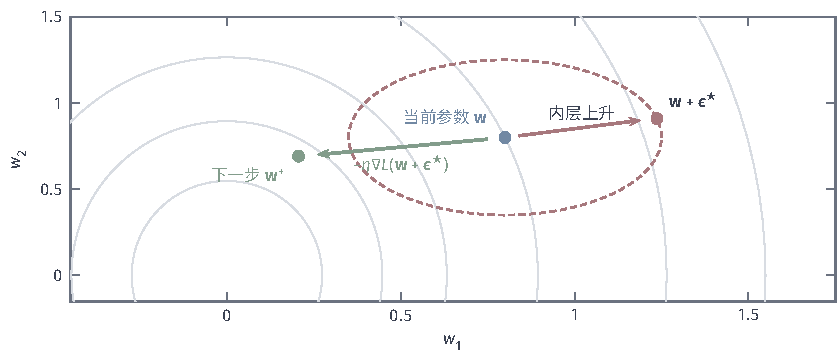
\includegraphics[width=142.275mm]{figures/05-neural-network-models/00-shared/tikz/generalization-sam/figure.pdf}
  \caption{SAM一次近似更新的几何过程。灰线为教学目标$L(\bm w)=(4w_1^2+w_2^2)/2$的等高线，红色虚线是以当前参数为中心、半径$\rho=0.45$的扰动邻域。红箭头沿当前梯度的一阶近似到达边界高损失点，绿色箭头使用该扰动点的梯度更新原参数。图示说明两次梯度读取及更新的位置；内层只采用一阶近似，泛化效果另在任务上评价。}
  \label{fig:generalization-sam}
\end{figure*}

SAM在指定参数坐标和范数下改变邻域目标，重参数化也会改变同一函数的扰动集合。$\rho$很小时更新接近普通梯度，较大时一阶近似可能失准或妨碍拟合。这里扰动参数，输入鲁棒训练则扰动样本，两者评价的邻域不同。两次前后向的成本、训练拟合与独立验证风险一起说明该目标是否适合当前任务\scite{foret2021sam}

\subsection{权重衰减}
\label{sec:generalization-weight-decay}

当前位置的梯度给出数据损失方向，还可以在同一次更新中缩小参数幅度。\term{权重衰减}（weight decay）直接加入这种参数收缩；通常将学习率与衰减系数的乘积限制在零与一之间。第\ref{sec:training-optimizers}节的方向、尺度与历史状态共同决定它是否等价于损失中的范数惩罚。对无动量的普通SGD，L2惩罚更新为
\begin{equation}
  \bm\theta^{(t)}=\bm\theta^{(t-1)}-
    \eta_t(\bm g^{(t)}+\lambda\bm\theta^{(t-1)})
  =(1-\eta_t\lambda)\bm\theta^{(t-1)}-\eta_t\bm g^{(t)}\text{。}
  \label{eq:generalization-sgd-weight-decay}
\end{equation}
因而在相同参数范围及系数约定下，L2惩罚与学习率乘以$\lambda$的收缩等价。若所谓“衰减系数”直接表示每步乘法系数，就还需对应学习率；加入动量后，惩罚是否进入缓冲会改变下一步方向，等价关系据该实现重新对应。

对预条件矩阵$\bm P^{(t)}$，惩罚项进入梯度后产生$-\eta_t\lambda\bm P^{(t)}\bm\theta$，而解耦收缩产生$-\eta_t\lambda\bm\theta$。二者通常不同，Adam中惩罚还可能进入一阶、二阶矩统计。\term{AdamW}将衰减从自适应梯度更新中分离，其基本更新为
\begin{equation}
  \bm\theta^{(t)}=(1-\eta_t\lambda)\bm\theta^{(t-1)}-
    \eta_t\frac{\hat{\bm m}^{(t)}}{\sqrt{\hat{\bm v}^{(t)}}+\epsilon}\text{，}
  \label{eq:generalization-adamw}
\end{equation}
这里矩统计来自数据损失梯度，具体计算见式\eqref{eq:training-adam}\scite{loshchilov2019adamw}

衰减通过多步乘积发生，学习率调度、更新次数和是否排除部分参数都会改变总收缩量。解耦项按原参数直接收缩，预条件后的惩罚梯度则使用另一个方向。比较强度时同时固定更新规则与系数含义。

\subsection{Dropout}
\label{sec:generalization-dropout}
\label{sec:generalization-stochastic-regularization}

分类器若总依赖同一组中间特征共同出现，可以在训练中随机屏蔽其中一些，要求剩余特征仍参与预测。共享参数由这些随机计算共同训练，因而接受不同可用路径下的监督。\term{Dropout}在训练时随机屏蔽部分激活，使网络在不同的可用特征子集上完成同一任务。设隐藏表示为$\bm h$，各元素独立保留概率为$q\in(0,1]$，$m_j\sim\operatorname{Bernoulli}(q)$。常见的反向缩放形式为
\begin{equation}
  \tilde h_j=\frac{m_j}{q}h_j,\qquad
  \mathbb E[\tilde h_j\mid\bm h]=h_j,\qquad
  \operatorname{Var}(\tilde h_j\mid\bm h)=\frac{1-q}{q}h_j^2\text{。}
  \label{eq:generalization-dropout}
\end{equation}
训练时除以$q$，常规推理时关闭屏蔽并直接使用$\bm h$。另一约定在训练时不缩放、推理时乘$q$，两者必须与实现一致。这里$q$为保留率，有些接口使用的是失活率$1-q$\scite{srivastava2014dropout}

训练目标包含对掩码的期望$\mathbb E_{\bm m}\ell(f_{\bm\theta,\bm m}(\bm x),y)$。各掩码产生的子网络共享参数，梯度共同更新同一组对象。隐藏表示的期望虽被保持，完整非线性映射一般不满足$\mathbb E_{\bm m}f_{\bm\theta,\bm m}=f_{\bm\theta}$；无掩码推理提供确定计算，对随机网络平均的解释采用近似。

图~\ref{fig:generalization-dropout}展示同一隐藏层的一个掩码样本。被屏蔽单元的输入参数仍保留，后续批量可以重新启用该路径。较低$q$增加扰动和方差，也可能损害拟合。BatchNorm与Dropout组合时，还需关注随机激活对运行统计的影响；序列模型中跨时间独立采样或共享掩码，则具有不同扰动结构。
\begin{figure}[htbp]
  \centering
  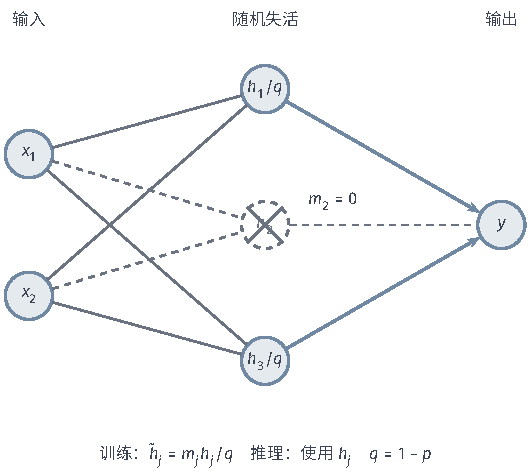
\includegraphics[width=89.793mm]{figures/05-neural-network-models/00-shared/tikz/generalization-dropout/figure.pdf}
  \caption{一个三单元隐藏层的构造性Dropout示意。中间单元保留浅灰$h_2$轮廓并标出$m_2=0$，表示本批屏蔽的单元仍保留在模型中；灰色虚线为本次不参与前向计算的路径。底部公式带明确区分保留概率$q=1-p$与丢弃概率$p$，并给出inverted Dropout在训练时除以$q$、推理时无需再缩放的约定。}
  \label{fig:generalization-dropout}
\end{figure}

\subsection{结构化随机失活}
\label{sec:generalization-structured-dropout}

随机扰动应覆盖模型真正依赖的信息单位；若重复线索能从邻近位置轻易补回，逐元素屏蔽施加的约束就较弱。结构化随机失活根据网络结构选择连接、通道、空间块或整层作为屏蔽对象，使扰动粒度与第\ref{sec:training-connections}节的结构组织对应。

\term{DropConnect}对权重连接采样掩码，令$\tilde{\bm W}=\bm M\odot\bm W$，随后再计算激活；Dropout则直接作用于激活。基本训练与推理的缩放、分布近似应按各自约定处理，两种失活的随机函数不相同\scite{wan2013dropconnect}

\term{空间Dropout}（spatial dropout）在一个通道的所有空间位置使用同一掩码，削弱网络对某个整通道特征的依赖。\term{DropBlock}随机屏蔽特征图中连续的空间块，干扰局部邻域可提供的重复信息。多个块会重叠，边界也截掉部分位置，因此块中心的采样概率与最终元素失活比例需要分别计算\scite{ghiasi2018dropblock}

\term{随机深度}（stochastic depth）对残差分支随机启用或绕过，让训练时经过的有效深度变化。一个期望保持的实现写为$\bm h^{(l+1)}=\bm h^{(l)}+(m_l/q_l)F_l(\bm h^{(l)})$，$m_l\sim\operatorname{Bernoulli}(q_l)$，推理时使用全部分支。原始方法也可将缩放放在推理阶段；是否真正跳过被屏蔽分支的计算影响训练时间\scite{huang2016stochasticdepth}

连接、通道、空间块和整层使不同信息共同失活。小对象、窄通道或缺少恒等路径时，大块屏蔽可能直接去掉任务证据。保留概率、作用位置与掩码共享范围共同确定扰动，再据实际结构和验证结果选择其强度。

\subsection{噪声注入}
\label{sec:generalization-noise}

除保留或屏蔽之外，还可以连续改变表示或参数，在规定扰动分布下训练其平均表现。参数分布与期望损失提供这一描述的理论接口（参考\BookSectionRef{sec:parameter-distributions}{第二卷“基础、理论和可信性”的“深度学习的可学习性”章“基于参数分布的可学习性”节}）。\term{噪声注入}（noise injection）在训练中使用$\tilde{\bm h}=\bm h+\bm\epsilon$或$\tilde{\bm\theta}=\bm\theta+\bm\epsilon$，其中噪声的均值、协方差和采样范围需要明确。输入噪声属于数据增强的一种，中间表示噪声改变后续计算，参数噪声则同时影响所有使用该参数的位置。

对足够光滑的目标函数和小幅零均值噪声，二阶展开给出局部近似
\begin{equation}
  \mathbb E_{\bm\epsilon}[\mathcal L(\bm\theta+\bm\epsilon)]
  \approx\mathcal L(\bm\theta)+\tfrac12
      \operatorname{tr}(\bm\Sigma\nabla^2\mathcal L(\bm\theta))\text{，}
  \label{eq:generalization-noise-expansion}
\end{equation}
其中$\bm\Sigma=\mathbb E[\bm\epsilon\bm\epsilon^{\top}]$。噪声幅度与光滑条件控制余项，协方差与当前Hessian共同决定二阶项；非凸区域的负曲率还可能使该项为负。

一个可精确核查的特殊情况是线性回归。给定当前样本，对预测$\bm w^{\top}\bm x$、平方损失及输入噪声$\mathbb E\bm\epsilon=\bm0$、$\mathbb E\bm\epsilon\bm\epsilon^{\top}=\sigma^2\bm I$，有
\begin{equation}
  \mathbb E\tfrac12[y-\bm w^{\top}(\bm x+\bm\epsilon)]^2
  =\tfrac12(y-\bm w^{\top}\bm x)^2+\tfrac{\sigma^2}{2}\lVert\bm w\rVert_2^2\text{。}
  \label{eq:generalization-linear-noise}
\end{equation}
零均值消去交叉项，协方差决定额外二次项。这份精确联系来自线性预测、平方损失与输入噪声，改变模型、损失或注入位置后，期望目标需按新计算展开。

Dropout也可理解为一种乘性噪声：$\tilde h_j=h_j+[m_j/q-1]h_j$，条件均值为0、方差与$h_j^2$成比例。它与加性高斯噪声的分布和尺度不同。噪声是否符合任务中合理的变化，决定了对局部邻域的约束是否有意义；系统性错误标签或数据泄漏则仍需修正监督与数据组织。

\section{模型集成}
\label{sec:generalization-ensembles}

若不同训练过程保留了不同预测误差，可以通过组合预测减少其中部分波动。第\ref{sec:generalization-solution-selection}节的解差异在这里进入组合，成员质量与误差相关性共同决定效果。

\subsection{装袋法（Bagging）}
\label{sec:generalization-bagging}

\term{装袋法}（bootstrap aggregating, Bagging）从训练集多次自助重采样，分别训练成员，再组合预测，第\ref{sec:ensemble-bagging-bootstrap}节给出采样机制。变化的样本集合形成不同解，预测组合尝试减弱单次采样的影响。这里也关心学习过程的抽样敏感性，算法稳定性则在指定假设下分析替换样本对损失的影响（参考\BookSectionRef{sec:algorithmic-stability}{第二卷“基础、理论和可信性”的“一般学习的可学习性”章“算法稳定性与可学习性”节}）。用神经网络作为成员时，仍需保持相同的输出语义：回归平均数值预测，分类可平均类别概率或投票；概率平均通常不等于先平均分数再做Softmax。组合规则见第\ref{sec:ensemble-members-combination-output}节\scite{breiman1996bagging}

重采样的覆盖率和袋外预测分别由式\eqref{eq:ensemble-oob-probability}与式\eqref{eq:ensemble-oob-prediction}说明。神经网络的超参数和成员由验证选择，相关数据再按实际抽样单位重采样。例如按主体抽取体现主体变化，按窗口抽取则体现另一种随机过程。

集成收益还取决于成员之间共享多少波动。式\eqref{eq:ensemble-correlated-variance}在固定输入、等方差和等相关条件下，描述标量预测平均的方差，随机性来自训练集抽取、重采样及训练过程。共同波动在平均中继续保留，偏差还由成员的期望预测决定。这份标量预测方差公式解释波动，分类零一风险则还取决于目标与决策边界。

\subsection{基于训练随机性的集成}
\label{sec:generalization-randomness-ensemble}

初始化、数据次序、增强和随机失活在同一训练集上也能形成不同预测函数，来源见第\ref{sec:generalization-solution-selection}节。使用这些训练选择构建集成时，差异来自过程，成员可以使用相同原始样本。袋外集合则需要装袋法中未抽中的样本这一数据组织。

成员质量与差异共同进入组合。在关键输入上系统性错误的模型可能拖低预测，几乎相同的模型则保留共同误差。单模型表现、预测分歧与组合权重由同一验证方案比较，确定成员后再做最终测试。

集成通常增加训练和推理成本。$M$个相同规模网络若顺序运行，模型计算量约为单个的$M$倍；并行运行可以降低部分等待时间，却需要更多设备或存储。第\ref{sec:generalization-weight-averaging}节的参数平均形成一个模型，预测集成则保留多个模型；前者在平均参数上重新计算，后者组合已有输出，函数与部署成本都可能不同。成员数与组合规则据任务质量、延迟和资源预算共同选择。

\section{本章小结}
\label{sec:generalization-summary}

相同训练拟合可以依赖不同线索，未来使用时的风险因而需要连同数据覆盖、结构偏好与选解过程判断。同分布新样本、场景变化和持续状态各有评价条件，数据划分据实际使用方式组织。

增强把任务允许的变化写进经验目标，参数共享与范数惩罚引入结构和尺度偏好，权重衰减通过更新收缩参数，随机失活与噪声约束受扰动的计算，停止时刻和参数平均改变轨迹上的解选择，集成则利用多个预测的差异。组合时各自条件仍起作用：增强保持任务语义，约束保留所需规律，参数平均保持坐标对应，集成成员提供合适差异。复杂度、稳定性与隐式偏差解释其中不同环节，符合使用场景的验证与独立测试再检验完整方案。

\paragraph{扩展阅读}
Goodfellow等教材第7章讨论显式与隐式正则化；Mixup原论文展示如何把样本间的插值约束加入训练。阅读时可将增强的任务语义、更新路径与预测评价接在一起，辨认各结果使用的数据与条件\scite{goodfellow2016,zhang2018mixup}
